\author{Team Simulus}
\title{7CCSMGPR Final Report}
\date{26/03/2015}
\documentclass[11pt,a4paper]{article}

\usepackage[utf8]{inputenc}
\usepackage{amsmath}
\usepackage{amsfonts}
\usepackage{amssymb}
\usepackage{graphicx}
\usepackage{fancyhdr}
\usepackage{wrapfig}
\usepackage{enumitem}
\usepackage{pgfplots}

%--- Settings for Java code snippets ---
\usepackage{listings} 
\usepackage{color}

\definecolor{dkgreen}{rgb}{0,0.6,0}
\definecolor{gray}{rgb}{0.5,0.5,0.5}
\definecolor{mauve}{rgb}{0.58,0,0.82}

\lstset{frame=tb,
  language=Java,
  aboveskip=3mm,
  belowskip=3mm,
  showstringspaces=false,
  columns=flexible,
  basicstyle={\small\ttfamily},
  numbers=none,
  numberstyle=\tiny\color{gray},
  keywordstyle=\color{blue},
  commentstyle=\color{dkgreen},
  stringstyle=\color{mauve},
  breaklines=true,
  breakatwhitespace=true,
  tabsize=3
}
%--- Settings for XML code snippets ---
\definecolor{lightgray}{rgb}{.9,.9,.9}
\definecolor{darkgray}{rgb}{.4,.4,.4}
\definecolor{forestGreen}{RGB}{34,139,34}
\definecolor{maroon}{rgb}{0.5, 0.0, 0.0}

\lstdefinestyle{XMLStyle}{
language=XML,
%Formatting
basicstyle=\scriptsize,
sensitive=true,
showstringspaces=false,
numbers=left,
numberstyle=\tiny,
tabsize=4,
numbersep=3pt,
extendedchars=true,
xleftmargin=2em,
lineskip=1pt,
breaklines,
captionpos=t,
%Coloring
backgroundcolor=\color{lightgray},
morekeywords={BooleanExpression},
alsoletter={:,,?},
morestring=[b]{"},
morecomment=[s]{<!--}{-->},
keywordstyle=\color{forestGreen},
identifierstyle=\color{maroon}\ttfamily,
stringstyle=\color{blue}\ttfamily,
commentstyle=\color{forestGreen}\ttfamily
}

\lstdefinelanguage{xml}{
basicstyle=\small,
sensitive=false,
}

\lstnewenvironment{xml-code}[2]{
\lstset{caption=#1,label=#2,style=XMLStyle}
}{}

%-- Plots ---
\pgfplotsset{width=10cm,compat=1.9}
\usepgfplotslibrary{external}
\tikzexternalize

%--- Page style ---
\pagestyle{fancy}
\fancyhf{}
\fancyhead[L]{7CCSMGPR Final Report}
\fancyhead[R]{Team Simulus}
\fancyfoot[C]{\thepage}

\begin{document}
	\section{Introduction}
With the development and growth of cities comes an increase in traffic volume and congestion. Traffic congestion can be explained generally as a decrease of road availability or an increase in vehicle volume that causes traffic to flow more slowly. The effects of congestion cost the economy billions of pounds each year in delays and wasted time \cite{arnott1994economics,FinancialTimes}, with these costs on an expected rise year on year. 

A main strategy for dealing with congestion is to manage traffic by introducing road policies that spread traffic more evenly over a network of roads. The idea is that introducing a speed limit or imposing a toll in an area with high traffic congestion will effectively cause that area to be less congested over time \cite{TFLImpacts}. More often, however, new road infrastructure must be introduced to solve these problems.

\subsection*{Problem Definition}
The construction of new roads is extremely expensive \cite{BBC}, and as such, it is important to ensure that any new road systems or changes to existing infrastructure will have the desired impact on congestion. Traffic simulation software enables the modelling of road infrastructure and traffic, along with the analysis of varying levels of traffic volume and the effects of different traffic management policies on the modelled infrastructure. This type of software is becoming an increasingly important tool for transport system analysis and management because it allows the modelling of a real-world scenario where a trial and error approach is simply infeasible. At the operational level, it permits a traffic engineer to evaluate and study the performance of a transport network under a plethora of alternative management options \cite{hidas2002modelling}.

\subsection*{Approach}
In this report, we document the construction of traffic simulation software over a short period of time by a small team of five developers.
The resulting software system is comprised of a simulator and an editor. The editor part of the system allows a user to design the road infrastructure which can then be executed by, and analysed within, the simulator. 

In section 2, we review various relevant literature associated with traffic simulation as well existing related works. Section 3 is associated with the description of the requirements specification pertaining to both the editor and simulator applications based on the conducted research. We also explain the design decisions of the Graphical User Interface (GUI) as well as software architecture. In section 4, we highlight the hurdles faced in the implementation of both software artefacts and the ways in which they were overcome. We then describe the extent to which the simulation was tested in, and the implications that this reality holds on the quality of our software. We discuss the ways in which we collaborated as a team in section 5, and the strategies and tools we implemented for decision making and communication. Finally, in section 6 we evaluate the software development process and draw conclusions about the project holistically. 
	\section{Review}
There are many variations on traffic simulation modelling. Two of the most popular classifications of simulation models that are investigated are Microscopic and Macroscopic.

\paragraph{}
Macroscopic simulations employ mathematical models to simulate the overall flow of traffic. M.J. Lighthill likened the flow of traffic to the flow of liquid through a pipe and his early work with Whitham led to the LWR model which represents traffic solely as mathematical equations \cite{Lighthill1955Kinetic,Treiber2013Flow,6042479} ignoring individual vehicle behaviour completely in favour of more overall measures of traffic behaviour, such as flow and density \cite{boxill2000evaluation,ehlert2001reactive}. 

\paragraph{}
Microscopic simulations however, focus on individual vehicles. This gives a much more realistic model of traffic as in the real world each driver is an individual with differing temperament, behaviour and destination. Each vehicle in the simulation is therefore modelled individually, allowing different types of vehicles to be present, showing differing personality or logic applied to each one \cite{Owen:2000:STS:510378.510542}. Behaviour is governed by a set of valid real-world traffic policies and regulations \cite{Schulze:1997:UTS:268437.268764}, such as stopping at red lights and driving on the correct side of the road.
These individual vehicles are monitored as they interact with other vehicles and elements of the environment, such as traffic lights or stop signs.

\paragraph{}
Cellular automaton simulations are a relatively simple version of the microscopic model. Roads are comprised of a series of cells with vehicles moving from one cell to the next. One vehicle is assigned to one cell with the disadvantage being that all vehicles are assumed to occupy the same amount of space on the road \cite{Namekawa2005CellAutomaton,6737859}. These cellular simulations can be implemented, at the most basic level, by using an array equal to the number of cells, with a cell marked as either occupied or available.

\paragraph{}
Agent based systems are another method of creating microscopic models. Here the agents take the role of vehicles and are governed by a set of traffic rules and policies that dictate their actions. The agents will have a goal, usually a destination that they are required to reach, and will navigate to that goal by using sensory information that they gather from the environment and other agents, creating a very realistic depiction of individual driver behaviour \cite{948773,4621183}.

\pagebreak
Simulations can also be classified as continuous or discrete time models.
Continuous time models use differential equations to calculate the state of the model at a given time, with variables in the model corresponding to real values such as vehicles per mile \cite{Lighthill1955Kinetic}.
Discrete time models however may deal with time-slices or events. For time-slice models the simulation is split into constant time intervals, a vehicle's attribute values are then updated at each time slice \cite{Schulze:1997:UTS:268437.268764}. For event-orientated models a queue of events is scheduled to occur in order of time. These events represent a change of state within the model, for example a traffic light changing to red, or a car following another car would approximate the distance to the lead car and adjust its speed or acceleration appropriately \cite{Schulze:1997:UTS:268437.268764,algers1997review}.

\paragraph{}
Many traffic simulation models use 2D overhead views to give a visual representation of the simulation in action. Sewall et al. \cite{sewall2010continuum} developed a system for generating realistic 3D animations of large-scale traffic networks that is capable of simulating real-world traffic data in a believable manner. By using an extension of the continuum model of traffic flow they were able to model lane changes and merging of traffic. Comparisons on performance to the agent-based SUMO \cite{SUMO} system were favourable, showing an almost linear performance overhead with a large number of cars compared to the constant growth in overhead required by the SUMO system.

\paragraph{}
Traffic simulation does not apply only to vehicles; various studies have looked at pedestrian traffic models. Studies have found that large groups of pedestrians will naturally form lanes when moving that increase the speed at which they may travel; similarly a circular roundabout behaviour is demonstrated at intersections in order to maintain an efficient pace. These behaviours are comparable to how road traffic is directed and as such many similarities can be shared between pedestrian and vehicular traffic models \cite{helbing2001self,lovaas1994modeling,helbing2001traffic}.


	\section{Requirements}
	\section{Implementation}
In the following we want to describe implementation specific details of both the simulator as well as the map editing application. We will elucidate problems we faced during the implementation and the integration of both applications and how we solved them. 
\subsection{Simulator}
Behind the user interface of the simulator a continuously running thread is mandated with updating the current state of the simulation with each tick, i.e. every 50ms. The thread execution is triggered by the globally governing SimulationController and its \textit{run}-method (fig.~\ref{fig:animthread}) appears refreshingly simple. Despite the apparent simplicity the design of the thread posed a range of problems. As is usual for Java UI frameworks, JavaFX also prohibits changes to UI objects by any thread other the main application thread, forcing us to submit each update that is to be escalated to the interface as a \textit{runnable} object to said application thread's execution queue. To reduce scheduling overhead we kept the AnimationThread's main loop as simple as possible, resulting in no more than four calls to the mentioned execution queue. The calls to \textit{spawnRandomTrucks()} and \textit{spawnRandomCar()} depend on the car/truck-ratio currently present on the map, i.e. either one of the method is called depending on the current deviation from the desired ratio. The \textit{updateCharts()} method of the \textit{ControlsController} retrieves the statistics of the simulation from the map and adds a new data point to each of the charts. This is done in 500 millisecond intervals.

\begin{figure}[h]
	\begin{center}
		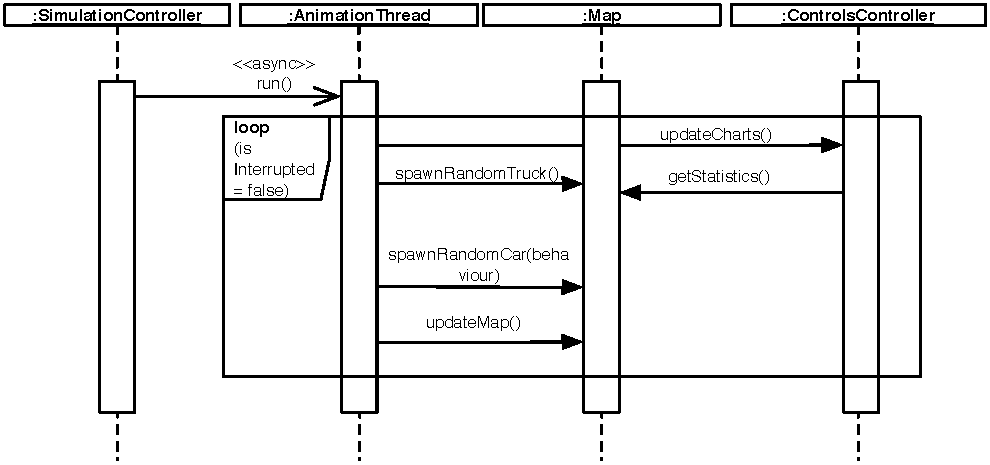
\includegraphics[width=\textwidth]{img/SD_animThread.pdf}
		\caption[Sequence Diagram of the Animation Thread]{Sequence Diagram of the Animation Thread}
		\label{fig:animthread}
	\end{center}
\end{figure}

With the multithreaded execution described above came concurrency related issues. The class Map contains a list to all vehicles currently present in the simulation. Whenever a vehicle is leaving the map, it notifies the SimulationController, which in turn removes the vehicle from the simulation. As the map's \textit{updateMap()} is constantly iterating through its list of vehicles, removing a vehicle from anywhere else than within this loop results in concurrency exceptions.

\begin{wrapfigure}{r}{0.45\textwidth}
	\begin{minipage}{0.45\textwidth}
		\begin{lstlisting}[caption={Car Removal}, label={lst:carRem}]
if(toBeRemoved.contains(v)){
	iter.remove();
	toBeRemoved.remove(v);
	continue;
}	
		\end{lstlisting}
	\end{minipage}
\end{wrapfigure}

In order to overcome this issue we considered both the traditional reader-writer-locking as well as the more advanced read-copy-update pattern, but eventually come to the conclusion but using either of them will introduce an additional scheduling (and implementation) overhead and hence only yield imperceptible performance improvements over the solution we employed (listing~\ref{lst:carRem}). As mentioned earlier, the \textit{updateMap()} method loops through all existing vehicles with each tick, we create a list of vehicles that are about to move the map within the next tick. As soon as the iterator (\textit{iter}) points to a vehicle \textit{v} that is on the \textit{toBeRemoved} list, it is removed and the loop skips one iteration.  

In order to ease the communication between model classes and the \textit{SimulationController} as well as the application classes \textit{MainApp} and \textit{EditorApp} we faced a design decision between the traditional observer pattern and the singleton pattern that allows static access to the required instances. We decided in favour of the singleton pattern, because the situations in which the model communicates with the \textit{SimulationController} are manifold and access to the singleton instance allows for fairly simple communication flows.

\subsection{Testing}
In order to meet all the requirements specified at the beginning of the project, testing forms an integral part in this process. Within the Agile development framework, we felt that Feature Driven Development (FDD) is most adaptable process suited for this project. Hence we decided to test the codes iteratively at the end of each development cycle. We foresaw that writing testing code in a concurrent fashion with the development team may not be an effective way, given the fact that the testing codes may not be working for the final product as incremental changes were made throughout the development. Therefore peer reviews were conducted at early stage to ensure  code quality is kept to standard, that is, each method should be written explicitly to address the problem that needs to be solved. In such manner, we can be assured of a rigid foundation (i.e. the software model) before we even attempt to adding more complicated features.

As the software becomes mature, unit tests were added to the project. We conducted unit testing in JUnit with the support of JemmyFX and ScenicView. JemmyFX is a third party library for testing JavaFX application. It is a test harness which allows the user to simulate user input, i.e. click buttons, entering data. In particular, JemmyFX defines how to get a list of scenes, nodes items, and get text of a \textit{javafx.scene.control.Label} (listing~\ref{lst:checkBox}). We have mainly used this for UI testing. 


\begin{minipage}{0.9\textwidth}
	\begin{lstlisting}[caption={Use JemmyFX syntax to find a checkBox element}, label={lst:checkBox}]

//Identifying the input checkBox element exist
assertEquals(CheckBox.class, new LabeledDock(scene.asParent(), checkBoxName, StringComparePolicy.EXACT).wrap().getControl().getClass());

//Find the label of the checkBox 
LabeledDock cb = new LabeledDock(scene.asParent(), checkBoxName, StringComparePolicy.EXACT);

	\end{lstlisting}
\end{minipage}

Using ScenicView helped us to understand what the UI was built from, allowing us and any other future developers to quickly and efficiently query the properties of a particular element, i.e. finding the properties of a JavaFX button (fig.~\ref{fig:scenicview}). ScenicView provides a tree structure and highlights the item upon it is selected. In the case of unable identifying an elements within the source code, this has been particularly helpful.  
\begin{figure}[h]
	\begin{center}
		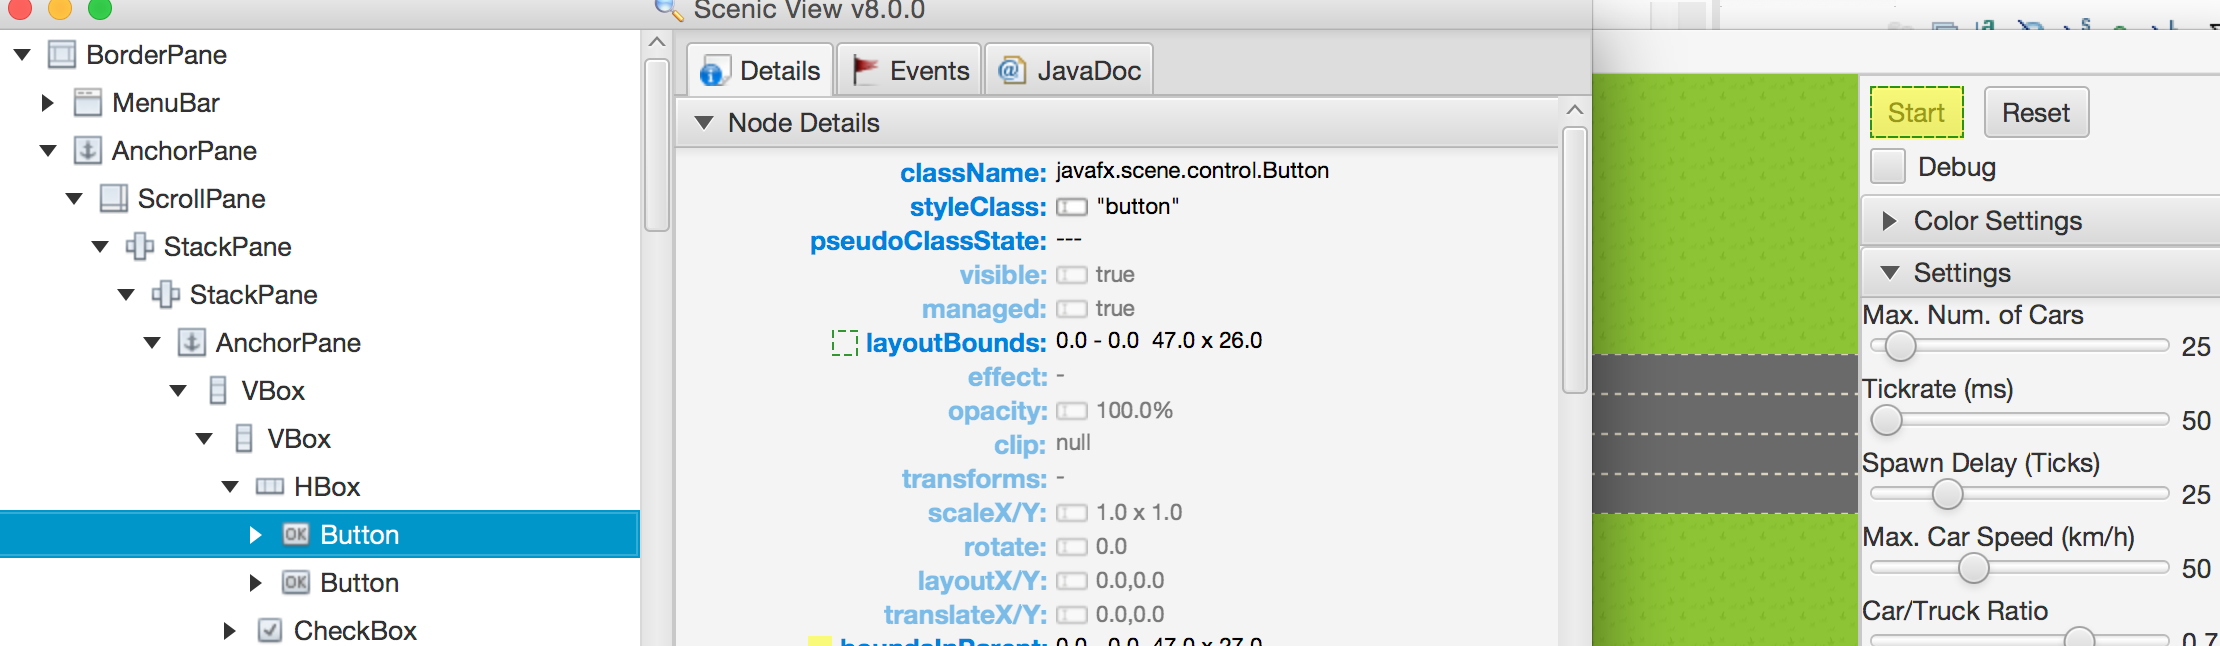
\includegraphics[width=\textwidth]{img/scenicView.png}
		\caption[Identifying properties of Start button with ScenicView]{Identifying properties of Start button with ScenicView}
		\label{fig:scenicview}
	\end{center}
\end{figure}

Since we were trying to achieve a multithreaded application, we reached a point where it was impossible to test every functionality due to the level of nesting and threading was too deep for us to comprehend. Therefore we focused our unit testing mainly on major components (i.e. vehicles, map and the model), in order to ensure features within them work correctly - in return that the application would behave accordingly. With such approach, this gives us the confidence that our code works as we expect it to work. 

It is arguably that there were lots of areas need to be tested. From one perspective, one could argue that the number of test cases could be used as an indication on the software quality. But we believed that unit testing is not about finding bugs. It is to prove that all the components could work together as a whole.  With this mentality, we carried out tests to ensure that the foundation of our code is dependable - at least within the scope of what this project aims to achieve.  

We wrote our test cases in an automated fashion. This allowed us to reduce the workload on manual testing.  A log was produced at the end for every test scenario. This also allowed us to identify problems should each scenario fails. An illustration is shown in fig.~\ref{fig:testCase}. 

\begin{figure}[h]
	\begin{center}
		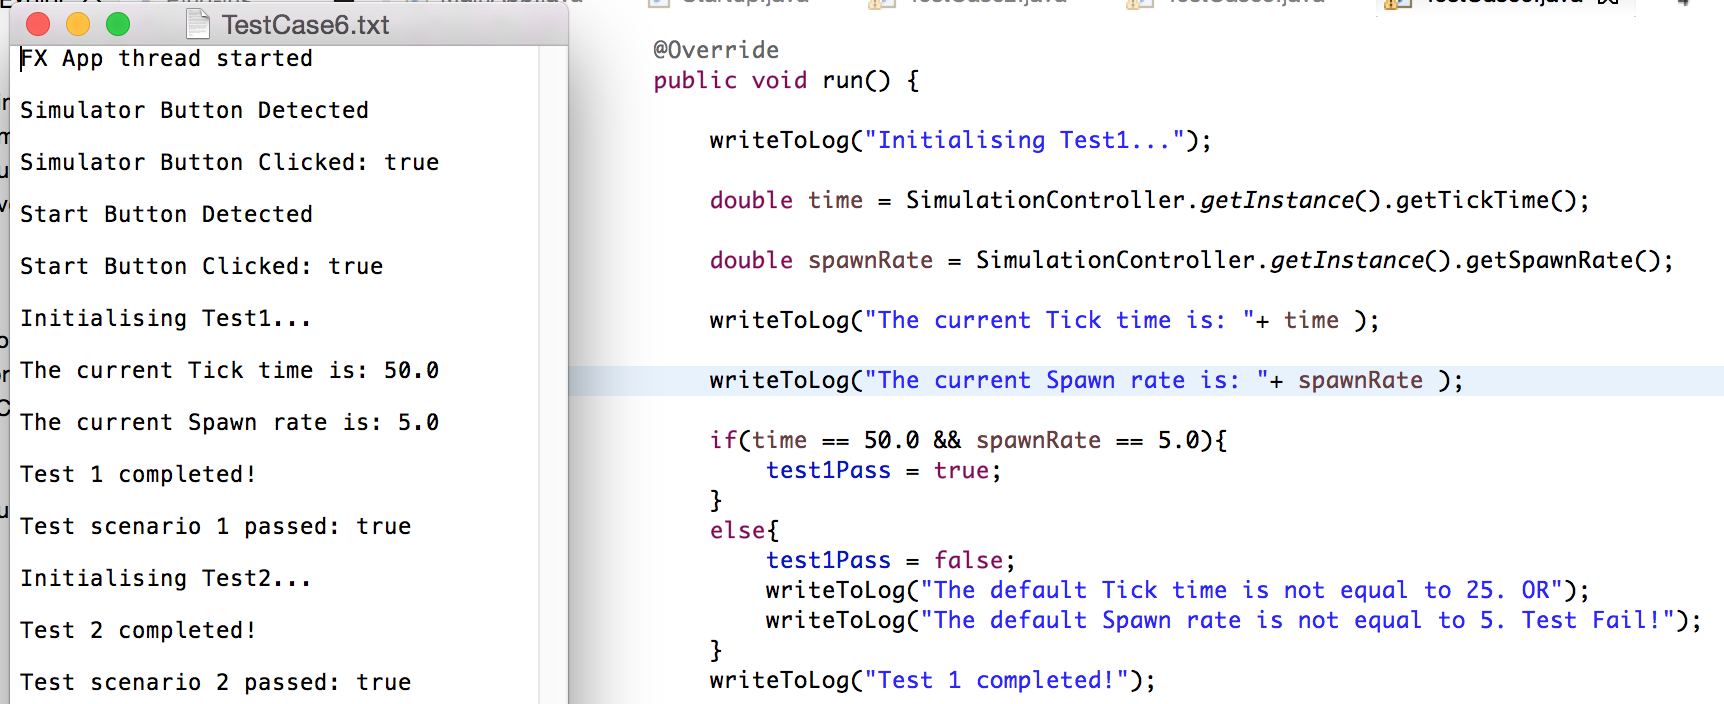
\includegraphics[width=\textwidth]{img/testCase.png}
		\caption{A log is produced after a test execution}
		\label{fig:testCase}
	\end{center}
\end{figure}

In addition, we also looked at the organisation of our code base to further assess the code quality of our software.  To do so we used a commercial tool to analyse the architecture. We produced diagrams such architectural dependencies, heat maps, UML Class Diagrams, as well as metric reports to give us a visual cue on the software internally. We then feed back the analysis to the development team in order to make changes accordingly. For instance, the heat map gave an indication on the level of \textit{lineCount} against \textit{maxCyclomaticComplexity}, as shown in fig.~\ref{fig:heatmap}. The bigger the shape it is the more lines of codes there have been written for a class. The colour depth of a shape indicates the density of its max complexity. At one stage, we identified the \textit{maxCyclomaticComplexity} for the \textit{Car.class} is 58, we were able to reduce it to 21 for the final version.     

\begin{figure}[h]
\begin{minipage}{\textwidth}
	\begin{center}
			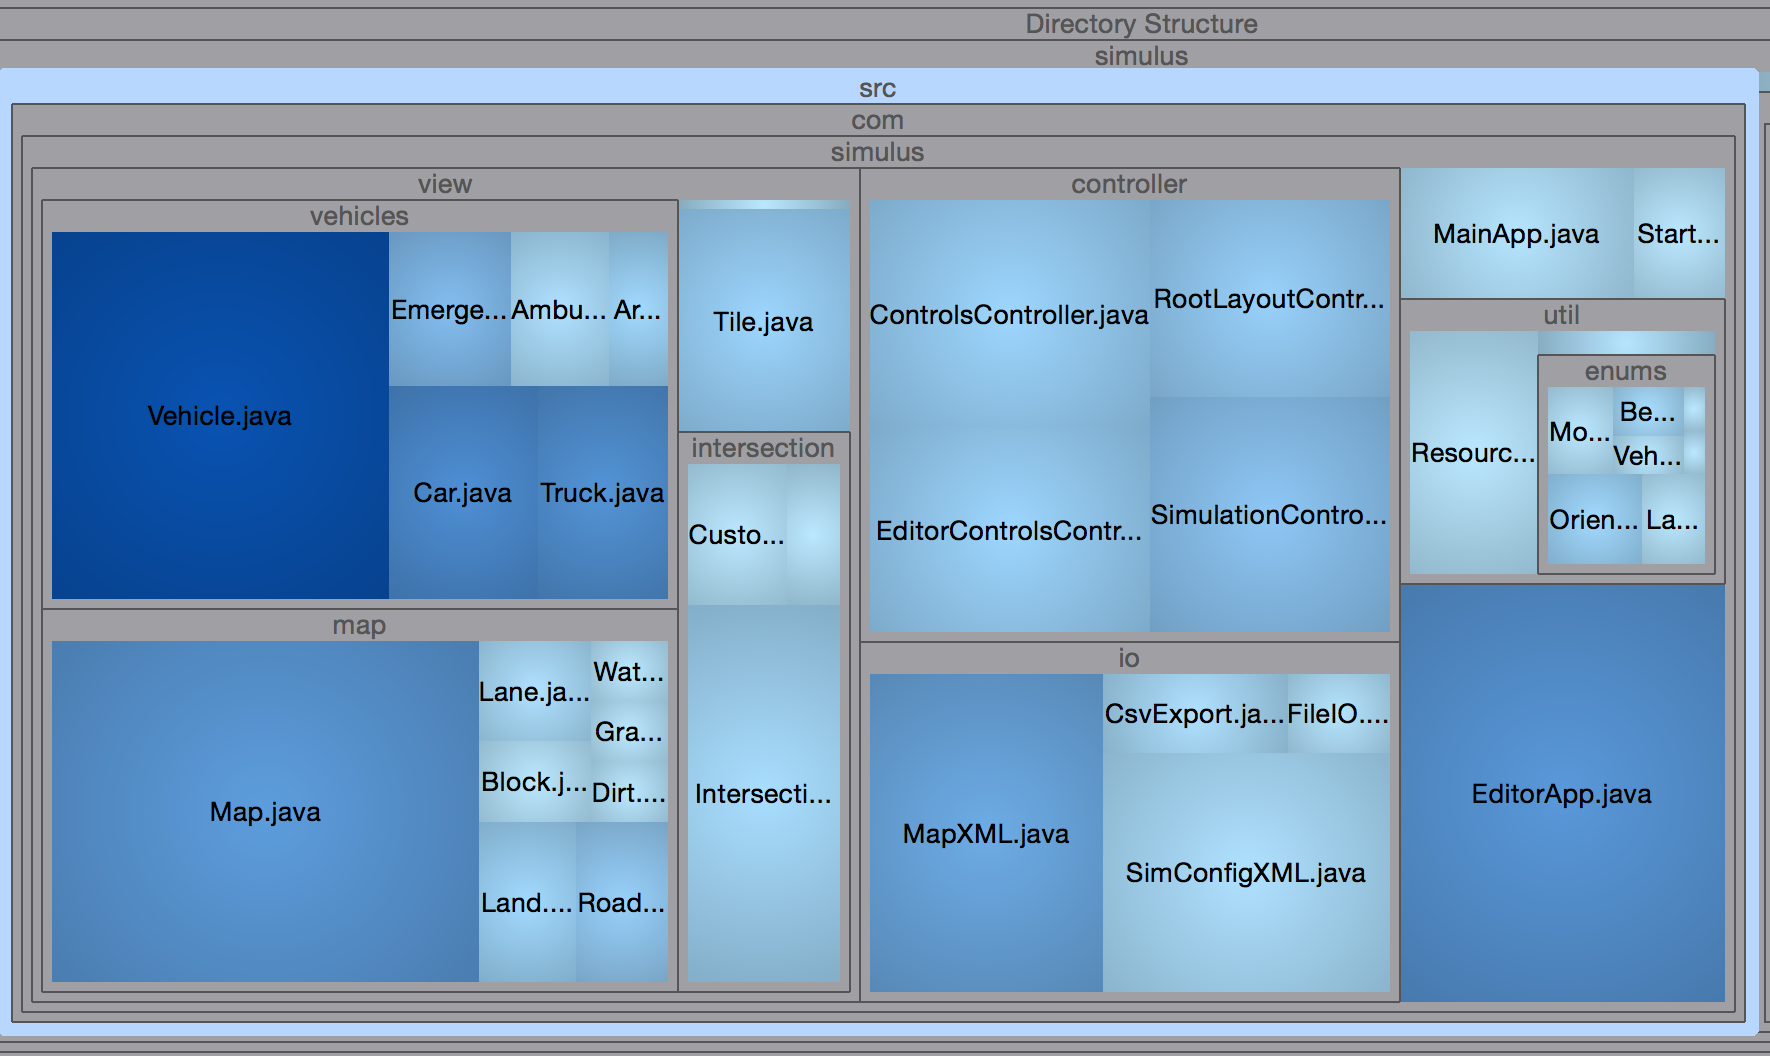
\includegraphics[width=71mm,keepaspectratio ]{img/heatmap.png}
		\caption{Heat Map for the final version of the software}
		\label{fig:heatmap}
	\end{center}
	\end{minipage}
\end{figure}

Fig.~\ref{fig:archIntDependency} illustrated the architectural dependency for our final product. We were assured that the outcome echoed to the requirement and design, though only a small portion of bi-directional calls were made internally. In most case, the architecture is preserved with uni-flow calls. There was no cluster found overall in this project, the architecture can be described more or less as clean, as shown in the figure. 

\begin{figure}[h]
	\begin{center}
			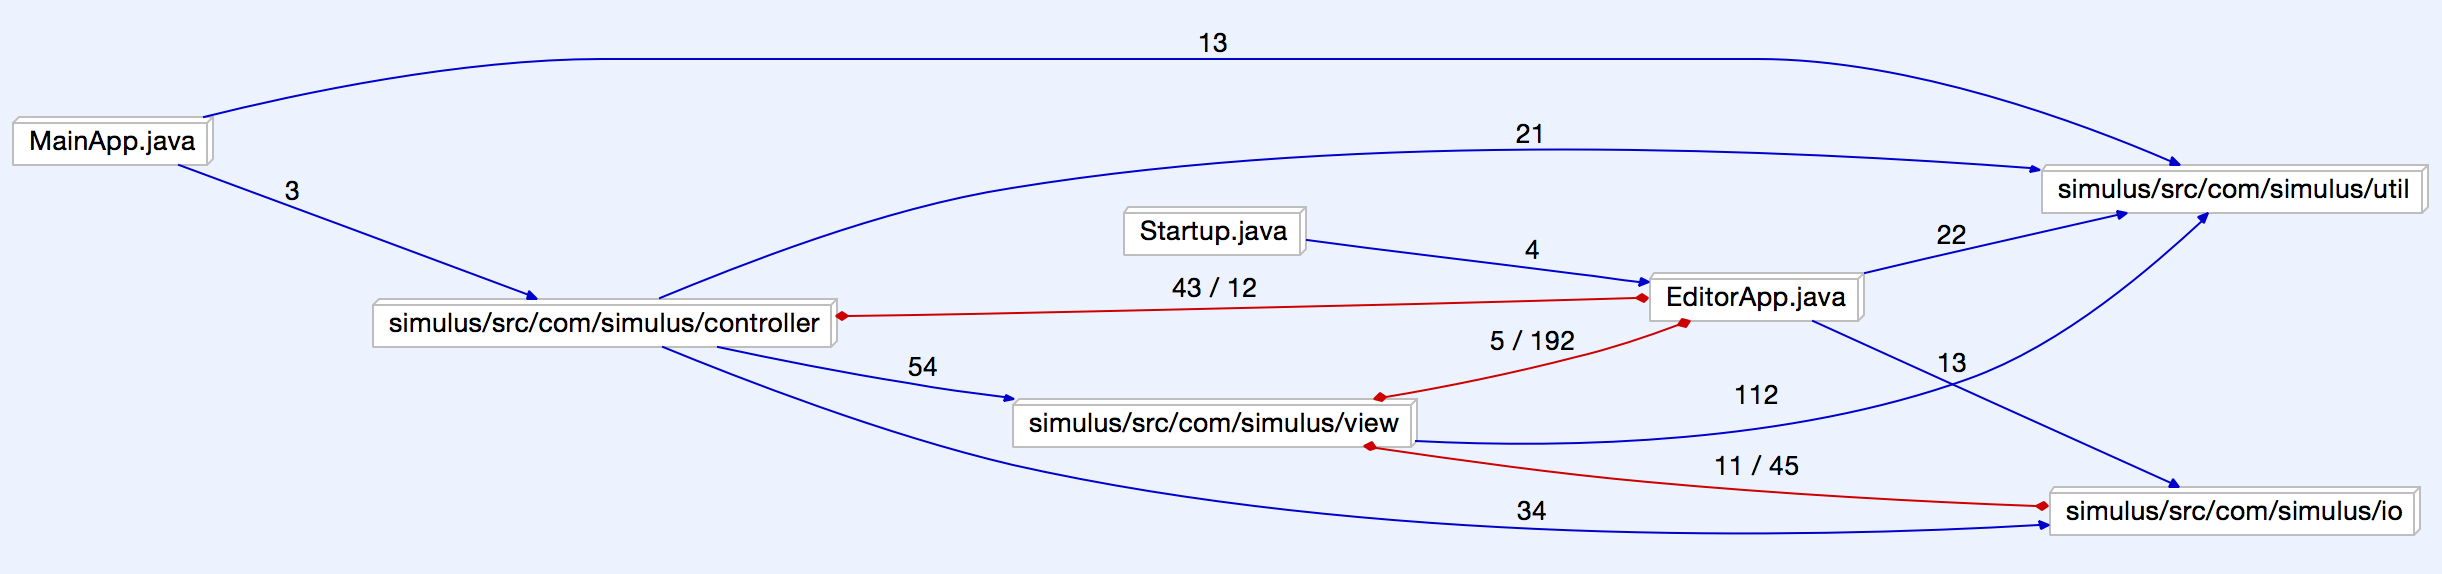
\includegraphics[width=\textwidth]{img/archIntDependency.png}
		\caption{Architecture Internal Dependency}
		\label{fig:archIntDependency}
	\end{center}
\end{figure}

\section{Map Editor}

\subsection{Graphical User Interface}
The majority of the effort with the editor application was on user interaction (UI) design and implementation. Recall the requirements from \ref{ss:req-editor} particularity those for usability (2.1-2.13). Fig.~\ref{fig:finalMapEditor} shows the resulting design chosen which the team felt had met the requirements in whole and one we hope is apparent when using the application to create a map.


\begin{figure}[h]
	\begin{center}
			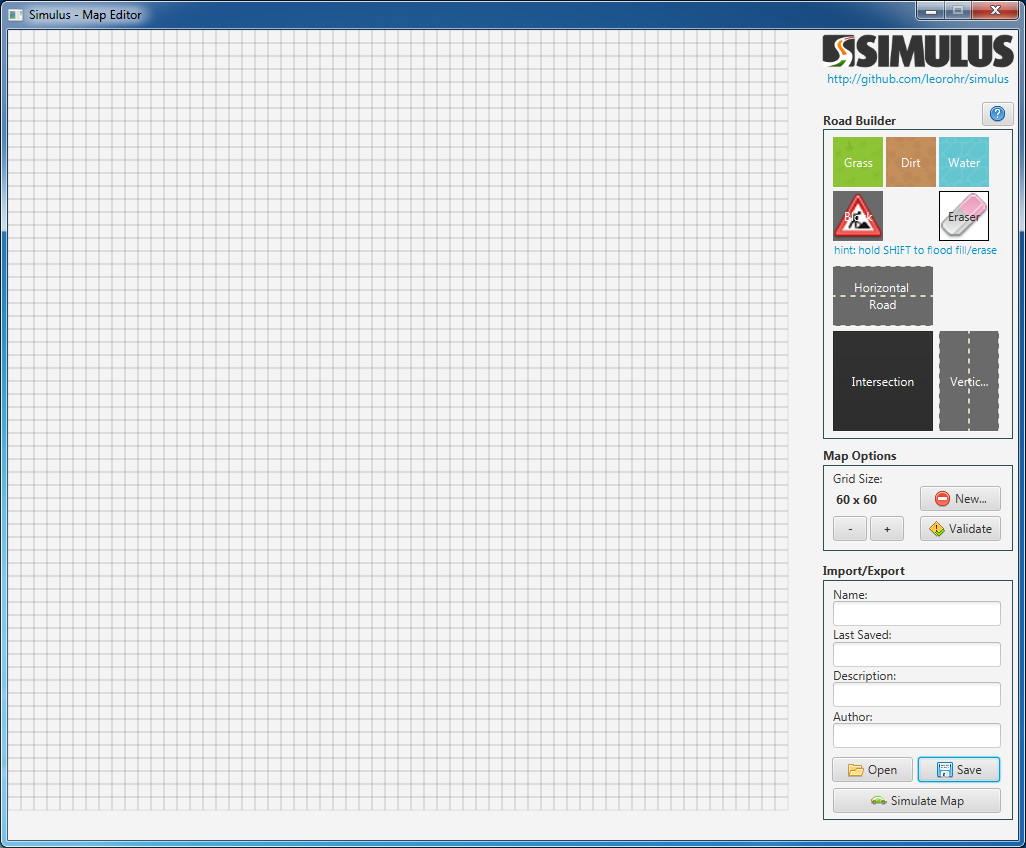
\includegraphics[scale=0.45]{img/mapEditorFinal.png}
		\caption{Resulting map editor design}
		\label{fig:finalMapEditor}
	\end{center}
\end{figure}

\subsection{Flood Fill}
The basis of any map editor is the ability to tag defined areas of desktop real-estate representing a real world instance e.g. land mass. We began by constructing an X*Y cell grid, where X and Y are the number of cells horizontally and vertically and where X=Y. The smallest instance of a map was to be a 40x40 grid yielding 1,600 tiles each needing to be individually tagged. Clearly it was not realistic to expect the user to tag each cell individually. Even when removing the number of tiles that would be tagged using the road and intersection tools, large swathes of the map are left unfilled.  
A method was required that would not only fill the remaining tiles with the users choice of texture but do so intelligently. That is only fill empty cells within in a certain boundary so as not replace existing ones.  This is is better known as a flood fill algorithm and is listed as requirement 2.7 and 2.8 of section \ref{ss:reqs}

There are several techniques for implementing flood fill (cite) of which the 4-way stack based implementation is seen as the simplest and most elegant approach due to its Depth First Search (DFS) recursive property.  The appropriate psudocode is as follows:

% probably need a new listing for psudocode?
\begin{minipage}{0.9\textwidth}
	\begin{lstlisting}[caption={4-way stack based recursive flood fill}, label={lst:stackFloodFill}]
Flood-fill (node, target-tile, replacement-tile):
1. If target-tile is equal to replacement-tile, return.
2. If the tile of node is not equal to target-tile, return.
3. Set the tile of node to replacement-tile.
4. Flood-fill (west of node, target-tile, replacement-tile).
   Flood-fill (east of node, target-tile, replacement-tile).
   Flood-fill (north of node, target-tile, replacement-tile).
   Flood-fill (south of node, target-tile, replacement-tile).
5. Return.
	\end{lstlisting}
\end{minipage}

This procedure was extended with bounds checking in our multidimensional array to give the observable results.

\begin{figure}[h]
	\begin{center}
		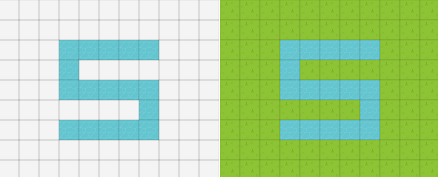
\includegraphics[scale=0.8]{img/floodFill.png}
		\caption[Flood Fill]{Before and after the use of flood fill}
		\label{fig:animthread}
	\end{center}
\end{figure}

Upon initial testing (ref. jerry's editor testing) the recursive approach performed exactly as expected with no functional issues  to report.  However, when the possibility of larger grid sizes was suggested, further testing revealed a fundamental flaw in this approach.  It was found that for a grid size larger than 65x65, a stack overflow would occur thus only partially filling the grid and causing the application to no longer respond.  With the ability to alter grid sizes implemented in later reversions of the simulator and editor applications, further investigation was warranted.

Approaching the literature, the stack over flow observation was commonly experienced and almost expected when using the recursive approach.  Mukherjee and Jana (2010, p.275) state:

 \begin{quotation}
A quick glance on the recursive variant of FloodFill function reveals that the recursive function makes four calls to itself at each step (for 4N connected region). Stack Overflow is the most common exception encountered while dealing with the recursive programs. Each time we call a function recursively, the function parameters, local variables and the return address of code (where to return when we are done with the recursion) are pushed to the stack. If the recursion is too deep, there may be overflowing of stack, where from there is no recovery.
 \end{quotation}
 
Possibly the simplest but least favoured approach was to alter the JVM's configuration parameters and increase the memory reserved for the stack.  Although this would be the simplest 'fix' it was not seen as a suitable solution given the many hardware and JVM configurations and further still, it was not a solution to the fundamental problem.

In the end the the recursive approach was deprecated while a 4-way queue based approach was implemented.  In contrast to the recursive implementation the queue based method is Breadth First Search (BFS) and uses a queue to store each new encountered tile.  The addition of two checks:

\begin{itemize}
  \item if the adjacent tile in question has not been already visited and
  \item if the tile is not of the target type
\end{itemize}

allowed for a tile to be added to the queue, replaced and dequeued in subsequent iterations. The relevant psudocode for the queue based approach is:

% probably need a new listing for psudocode?
\begin{minipage}{0.9\textwidth}
	\begin{lstlisting}[caption={4-way queue based flood fill}, label={lst:queueFloodFill}]
Flood-fill (node, target-tile, replacement-tile):
 1. If target-tile is equal to replacement-tile, return.
 2. Set Q to the empty queue.
 3. Add node to the end of Q.
 4. While Q is not empty: 
 5.     Set n equal to the last element of Q.
 6.     Remove last element from Q.
 7.     If the tile of n is equal to target-tile:
 8.         Set the tile of n to replacement-tile and mark 
 9			"n" as processed.
 10.        Add west node to end of Q if not yet processed.
 11.        Add east node to end of Q if not yet processed.
 12.        Add north node to end of Q if not yet processed.
 13.        Add south node to end of Q if not yet processed.
 14. Return.
	\end{lstlisting}
\end{minipage}

With this new revised function, grid size was no longer an issue and a flood fill of an empty 200x200 grid (larger than any suggested grid size) completed successfully without any noticeable delay.
\paragraph{}
To ensure the new approach would be indeed suitable for the set grid sizes, some simple measurements were taken.  The two algorithms were used to fill an empty grid with a 'grass' land tile, repeated three times and an average calculated.  The results shown in fig.\ref{fig:floodChart} clearly show that although the recursive stack based implementation performs on average 70\% faster, it was unable to function for grid widths greater than 60 in our set.  Although this may seem wholly a failure for the queue based implementation, it is important to point out that this equates to ~10ms difference. Not noticeable by any human operator.  Even more interesting was that the results quoted were based on First Time Run (FTR) values, immediately after launching the editor. Using the same two routines on subsequent occasions would yield repeated values as low as 10-16ms per fill.
 
\begin{figure}[h]
\centering
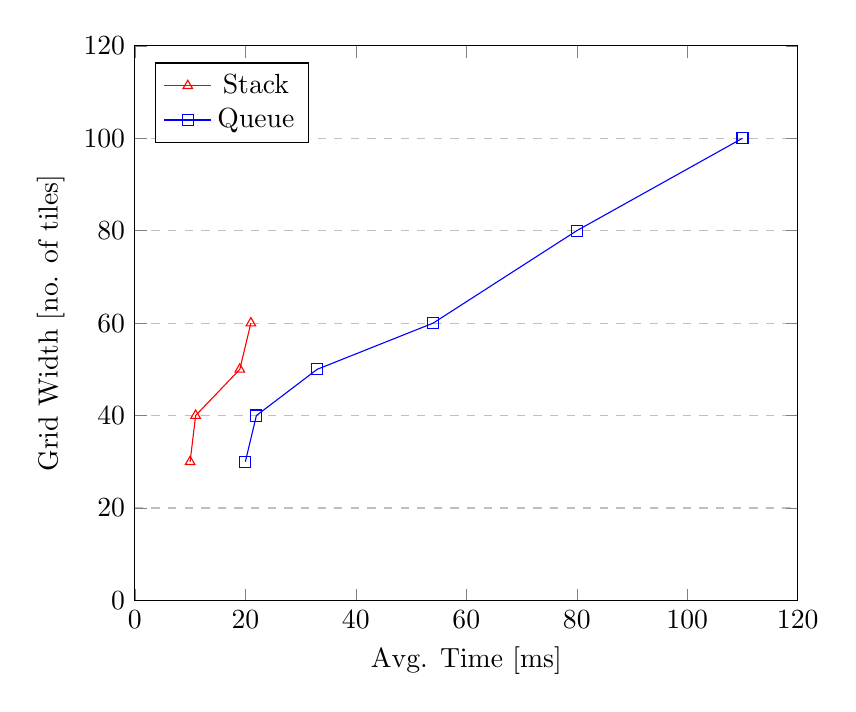
\begin{tikzpicture}
\begin{axis}[
    xlabel={Avg. Time [ms]},
    ylabel={Grid Width [no. of tiles]},
    xmin=0, xmax=120,
    ymin=0, ymax=120,
    xtick={0,20,40,60,80,100,120},
    ytick={0,20,40,60,80,100,120},
    legend pos=north west,
    ymajorgrids=true,
    grid style=dashed,
]
\addplot[
    color=red,
    mark=triangle,
    ]
    coordinates {
    (10,30)(11,40)(19,50)(21,60)
    };
\addplot[
    color=blue,
    mark=square,
    ]
    coordinates {
    (20,30)(22,40)(33,50)(54,60)(80,80)(110,100)
    };
    \legend{Stack, Queue}
\end{axis}
\end{tikzpicture}
\caption{Average execution time for flood fill}
\label{fig:floodChart}
\end{figure}

It must be noted that the new method is no longer as concise as a definition compared to the original but it was a subtle sacrifice for the benefits it yielded.
	\section{Team Work}
\label{sec:team_work}
Critical to the success of our project has been our ability to work as a collective with a clear objective, translated into practise by our organisation, use of tools and overcoming challenges when posed. We now focus on some of these aspects.

\subsection{Development Process}
As outlined in the initial report, we selected to follow an Iterative and Incremental Development (IID) process. This was evident in the group's Gantt chart (ref appendix) having planned short development cycles. These cycles comprised of a requirements and planning task to identify what was to be achieved and how it was to be accomplished. We then progressed to possible design solutions that would meet the requirements. We developed the feature and then carried out testing against it. Collectively evaluating the feature and our efforts in that week was the final stage of a cycle. Each feature had an exit point, where once the requirements where met, we could progress. In order to establish the priority for each feature and thus the order in which it would be implemented, the perceived value gained by each was our indicator wholly based on the MoSCoW analysis, carried out in section \ref{sec:reqs}.

A notable benefit of the above approach was that it encouraged modular design, facilitating deconstruction of large, undefined requirements into manageable features: "Map drawing feature" was refined to "land tiles have three different instances; grass, dirt and water" and "simulator has export button" to "there is the ability to export simulation parameters from within the simulator", etc.  
Probably the most beneficial aspect was that we were able to ascertain our development progress early on and thus adjust the time dedicated to the project, manoeuvring group members where additional effort was required. The iterative feedback not only allowed us to evaluate the software we were developing but our own techniques and group dynamics on a weekly basis.

\subsection{Team Policy}
The team's identified approach to management was wholly democratic opting to vote on most points of contention, from the triviality of tile colours to the more pressing decision of using a continuous model over the discrete prototype.

\begin{lstlisting}[caption={Decision Making Agreement}]
* Each individual has the opportunity to voice their concerns
* Each individual has an equal vote on an issue
* The majority vote is the deciding vote
\end{lstlisting}
 
Although one may have concern that this policy could lead to inaction, we found that system worked well for us on this occasion.  Perhaps this was in part due to the individual members, their personalities and working mentality. We had minimal, if any, conflicts to resolve, as a result of open discussion and brainstorming within the allocated weekly meetings and Facebook group.

\subsection{GitHub}
Our tool set for collaboration may seem inadequate at first glance, listing Facebook, WhatsApp and GitHub only. Upon closer inspection it is immediate that we fully embraced GitHub and most of it's available features. We have found GitHub to be an accomplished tool for software projects and can fully appreciate why it is popular in industry and open-source projects. For several of us, it was our first exposure to distributed version control and source code management but we can be confident that all facets of our group work was enhanced by the use of this tool.

The team's usage of GitHub was immediate but was largely adopted once we had made the decision to change to a continuous model.  Whereas previously we had worked in a single branch, we created an additional two - a 'model' and 'editor' for each area of the project.  This allowed the two development sub teams to work independently. At strategic points and at the end of a development cycle \ref{subsec:Development Process}, we would aim to merge the two branches with the necessary members present. As useful was the 'issues' feature where any individual may create a task for himself or for the team as a whole. We were able to translate functional requirements, to almost atomic levels in some cases, and assign them to team members. The ability to post questions and comments against an issue was helpful and the tagging feature became a handy method to quickly prioritise tasks. The team  did attempt to create suitable Wiki pages for the project but this was not entirely accomplished as expanded on in the next section.

\subsection{Challenges}
Inevitably we did face some challenges, none that were detrimental to the overall completion and achievement of our aims. However the basis of learning from our experience is that we are clear on what these were and how it was overcome. 

Having praised the value of using a Git repository in section \ref{subsec:GitHub}, it is important to understand that good communication is still paramount when working through such a system. Not being clear of the current classes a colleague is working on led to us on one occasion suffering a delay when a commit was made without reviewing the conflicts. Increased communication, through private messaging and the GitHub issues feature, meant this was no longer an issue once identified. All members made others aware of their current activity, progress and subsequent tasks to be tackled.

The team felt additional informational pages should have been posted to our Git's Wiki. An effort was made initially but not sufficiently to fully document the project. Unfortunately we were unable to find the time to make this a reality but it would be feasible to complete at a later date.

\todo refer to github (meeting minutes)

	\section{Evaluation}
\label{ss:eval_sim}
In terms of the realisation of initially set requirements, we were able to meet them all except for the inclusion of external map sources (requirement 3b in section~\ref{sec:reqs}). This, however, was associated with the "could have" priority class and hence is an acceptable shortcoming. As our map model is based on fixed sized tiles, it would require intense translation to reproduce a map from sources like Google Maps or KML files due to their high resolution. 

As described in section \ref{subsec:design}, we began using a discrete space model and changed to a continuous model later on. This change was a product of improved thinking, as we realised that the restrictions imposed by a discrete space representation outweigh the benefits of the easier implementation that comes with it.

At the beginning of the project we implemented a model-view-controller pattern. However, during the course of the implementation it became apparent, that strictly following this pattern is impractical for this particular project. In the current state of the software, the initially separated model and view are combined in the view package. An example for this consolidation are the vehicle classes. They extend the JavaFX class \textit{Rectangle}, which is used to visualise the different types of vehicles. Nonetheless, vehicles do also know their position in the map model and compute their movement on their own - both functionality that belongs to the model in a strict MVC architecture.

The methods that compute vehicle movements require numerous of checks for the vehicle's environment. An example would be the method by which a car overtakes another. Multiple tiles of the adjacent lane must first be checked for the conditions to be met for this manoeuvre to take place. The exact tiles that need to be checked currently depend on the direction of the vehicles' movement and hence these checks come with a lot of nested conditional statements. The \textit{attemptOvertake} method in the \textit{Vehicle} class exhibits a cyclomatic complexity of 34, therewith being the most complex method in our source code (see fig.~\ref{fig:heatmap}). Reducing the complexity for this method along with others would most likely improve the scaling of simulator performance with a higher number of vehicles. Implementing these changes would require a major redesign of the simulation logic and was hence deemed as infeasible to do within the short duration of this project.

Maps are persisted using the XML. Each map-file contains data for every single tile on the map. Unfortunately, the XML specification we used does not specify the grouping of tiles to an intersection, forcing us to recreate the intersections as soon as an intersection tile is encountered while reading the map. This means that the algorithm will create an intersection at the encountered tile and hence create the tiles 3 columns to the right and 3 rows down without reading any further tile information from the XML file. To ensure that intersections are created correctly, we have to create a 2D boolean array the size of the map (i.e. 40x40, 60x60 or 80x80) to keep track of tiles that have been loaded successfully. 

Our model currently only supports roads with four lanes and dual carriageways. As adding support for different lane models and road sizes will increase the capabilities and functionality of both simulator and editor, we consider this a suitable task for further development of the software. 

All five group members were involved in the creation of the code. Collaboration and communication was eased through extensive use of the Git Issues feature to track problems and progress in solving them (cf. section~\ref{sec:team_work}). Working in separate branches of the repository when working on the same files or related behaviour allowed every team member to contribute to the codebase continuously.  

\subsection{Future Work}
%evaluation of editor?

	\section{Peer Assessment}
	\appendix

\section{Appendix}

include schema for map, simulation parameters, csv export

meeting logs

gantt chart

gitlog
	
	\fancyfoot[C]{\thepage}
	\bibliographystyle{plain}
	\bibliography{literature}
\end{document}